\chapter{Propriété intellectuelle et clauses de non-concurrence}\label{ch:fm:intellectual-property-and-non-competes}

Le 5 juin 2009, son dernier jour chez Goldman Sachs, un programmeur qui avait travaillé sur le système de trading à haute fréquence de la banque a chiffré et téléversé
plus de 500\,000 lignes de son code source vers un serveur en Allemagne~; il avait accepté un poste dans une start-up qui développait son propre système de trading. Un jury
le déclara coupable au titre de deux lois fédérales, et il fut condamné à 97 mois de prison. En 2012, la cour d'appel du Second Circuit annula
les deux condamnations~: le code, jugea-t-elle, n'était pas un «~bien~» volé au sens de l'une des lois, et au regard de l'autre il ne se rapportait pas à un produit «~fabriqué
pour ou mis en circulation dans le commerce interétatique ou étranger~», la banque n'ayant vendu ni concédé sous licence son système de trading à personne. Dans l'année, le Congrès
modifia la seconde loi pour couvrir les produits et services utilisés dans le commerce. Les actifs les plus précieux d'une société de trading sont écrits dans du code et
portés dans la tête des gens, et le droit qui les protège tient à des mots de ce genre.

\section{Ce que possède une société de trading~: code, modèles, données et savoir-faire}

Le capital, les locaux et les relations d'une société de trading peuvent s'acheter. Ce qu'elle possède et qu'un concurrent ne peut pas acheter est un ensemble de choses difficiles à voir
et faciles à emporter~: code source, structure de ses modèles et de leurs paramètres calibrés, données nettoyées et jointes, journaux de recherche (livre~7)
consignant ce qui a été essayé et ce qui a échoué, et le savoir-faire de ceux qui les ont construits. La plupart de ces éléments ne sont protégés que de deux façons. Soit le droit
les tient pour un secret et punit leur soustraction, soit des contrats empêchent les personnes qui les connaissent de les utiliser ailleurs pendant un certain temps.

Les brevets et le droit d'auteur font peu de ce travail. Une stratégie de trading est rarement brevetable, et la breveter reviendrait à la publier~; le droit d'auteur protège le
texte du code mais non l'idée qu'il met en œuvre, et un concurrent qui réécrit un modèle de mémoire ne copie aucun texte. La protection de la société repose donc sur
le secret, et le secret est une question de degré~: chaque départ, chaque intervention en conférence et chaque prestataire qui voit les données en laisse fuir une partie.

Trois éléments diffèrent par la vitesse à laquelle ce qui fuit perd sa valeur.
\begin{itemize}
\item \textbf{La structure du modèle}~: les effets que la stratégie exploite et la manière dont elle les combine. Elle décroît lentement, au rythme de l'effet
lui-même~: l'encombrement (crowding) et la décroissance après publication (livre~7) l'érodent sur des années.
\item \textbf{Les paramètres}~: les poids, seuils et tailles calibrés. Leur valeur est élevée mais brève~: ils sont recalibrés tous les quelques mois, et
une copie périmée perd vite son edge.
\item \textbf{Les données}~: le pipeline qui nettoie et joint les entrées. Sa valeur décroît au rythme des propres évolutions des prestataires.
\end{itemize}
Le modèle du chapitre attribue à chacun une part des profits de la stratégie qu'un concurrent qui l'utiliserait s'approprierait, ainsi qu'une demi-vie, soit le temps que met la valeur de
ce qui a été pris à se réduire de moitié, c'est la demi-vie du signal du livre~7 appliquée au savoir fuité.

\section{Secrets des affaires et modes de protection}

\begin{definition}[Secret des affaires]\label{def:fm:intellectual-property-and-non-competes:secret}
Un \emph{secret des affaires}\index{secret des affaires} est une information, notamment du code source, des modèles et des données, qui n'est pas généralement connue ni aisément
vérifiable par d'autres acteurs du domaine, qui a une valeur commerciale parce qu'elle est secrète, et que son détenteur a pris des mesures
raisonnables pour la garder secrète.
\end{definition}

Les trois conditions sont presque identiques aux États-Unis, dans l'Union européenne et au Royaume-Uni (l'\cref{dat:fm:intellectual-property-and-non-competes:law}).
La troisième est celle qu'une société maîtrise, et celle autour de laquelle se joue le contentieux~: un juge demande ce que la société a fait, et non ce qu'elle voulait faire. Les mesures raisonnables
sont des contrôles ordinaires~: accès selon le principe du besoin d'en connaître, journalisation des copies et des téléversements, séparation des tâches (livre~6) entre ceux qui
écrivent le code et ceux qui peuvent le sortir des systèmes de la société, ainsi que les contrats.

\begin{definition}[Accord de confidentialité, clause de cession des inventions]\label{def:fm:intellectual-property-and-non-competes:nda}
Un \emph{accord de confidentialité}\index{accord de confidentialité} lie un salarié ou une contrepartie à ne pas divulguer ni utiliser les informations confidentielles de la
société, pendant et après la relation. Une \emph{clause de cession des inventions}\index{clause de cession des inventions} dans
un contrat de travail attribue à l'employeur les droits sur les travaux créés par le salarié dans le cadre de son emploi~: code, modèles, recherches et
documents.
\end{definition}

\begin{dated}{2026-09}{Droit du secret des affaires}\label{dat:fm:intellectual-property-and-non-competes:law}
\textbf{États-Unis}~: L'article 18 U.S.C. 1839(3) définit le \omterm{def:fm:intellectual-property-and-non-competes:secret}{secret des affaires} comme une information financière, commerciale, scientifique, technique, économique ou d'ingénierie
y compris les programmes et les codes, dont le détenteur a pris des mesures raisonnables pour la garder secrète et qui tire une valeur économique propre
du fait de n'être pas généralement connue ni aisément vérifiable. Le Defend Trade Secrets Act de 2016 (18 U.S.C. 1836) donne au détenteur une action civile fédérale,
avec une ordonnance de saisie civile disponible seulement dans des circonstances exceptionnelles, dans les trois ans suivant la découverte du détournement~;
l'infraction pénale du 18 U.S.C. 1832 s'applique, depuis le Theft of Trade Secrets Clarification Act de 2012, aux secrets liés à «~un produit ou
service utilisé ou destiné à être utilisé dans~» le commerce interétatique ou étranger. \textbf{Union européenne}~: la directive (UE) 2016/943, article~2, exige
que l'information soit secrète, qu'elle ait une valeur commerciale parce qu'elle est secrète et qu'elle ait fait l'objet de mesures raisonnables pour la garder secrète.
\textbf{Royaume-Uni}~: les Trade Secrets (Enforcement, etc.) Regulations 2018 (SI 2018/597) ont transposé les règles de la directive. Cet encadré est une
synthèse de textes publics, et non un conseil juridique.
\end{dated}

L'affaire pénale du hook montre pourquoi les mots comptent. La cour a jugé que le code source était immatériel, de sorte que son transfert par téléversement ne constituait pas
le transport d'un «~bien~» volé au sens du National Stolen Property Act~; et que le système de trading, que la banque gardait pour elle, n'était pas
un produit fabriqué pour ou mis en circulation dans le commerce interétatique, de sorte que l'Economic Espionage Act, dans sa rédaction d'alors, ne le visait pas. L'amendement de 2012 a remplacé
ces termes par un produit ou service «~utilisé ou destiné à être utilisé dans~» le commerce, ce qu'est un système de trading interne. L'action civile de 2016
a ajouté une voie fédérale pour le détenteur lui-même (la \cref{fig:fm:intellectual-property-and-non-competes:record}).

\section{Non-concurrence, garden leave et non-sollicitation}

Le droit du \omterm{def:fm:intellectual-property-and-non-competes:secret}{secret des affaires} agit après coup et doit prouver ce qui a été pris. Les contrats agissent en amont~: ils tiennent à l'écart du
marché, pendant un certain temps, les personnes qui connaissent le secret, qu'elles aient ou non emporté quelque chose.

\begin{definition}[Clause de non-concurrence, garden leave, clause de non-sollicitation]\label{def:fm:intellectual-property-and-non-competes:restrict}
Une \emph{clause de non-concurrence}\index{clause de non-concurrence} interdit à un ancien salarié de travailler pour un concurrent ou dans une activité définie, pendant une période
après son départ. Le \emph{garden leave}\index{garden leave} est une période de préavis pendant laquelle le salarié reste employé et rémunéré, mais tenu à l'écart
du travail, des clients et des marchés. Une \emph{clause de non-sollicitation}\index{clause de non-sollicitation} interdit à un ancien salarié de solliciter les clients de la
société ou débaucher son personnel pendant une période.
\end{definition}

Les deux restrictions diffèrent par celui qui paie et par la façon dont les tribunaux les apprécient. Le \omterm{def:fm:intellectual-property-and-non-competes:restrict}{garden leave} est un emploi rémunéré~: le salarié conserve son salaire et ses avantages, et
la restriction fait partie d'un préavis que le salarié a accepté. Une \omterm{def:fm:intellectual-property-and-non-competes:restrict}{clause de non-concurrence} prend effet après la fin du contrat~; certaines sociétés la rémunèrent, et certaines
juridictions l'exigent, et sa validité, ainsi que sa durée, dépend de la juridiction et des termes du contrat. Aux États-Unis
une interdiction fédérale a été annoncée en 2024 puis abandonnée en 2025 (l'\cref{dat:fm:intellectual-property-and-non-competes:ftc}). La \omterm{def:fm:hiring-and-compensation:deferral}{rémunération différée}
(chapitre~10) s'articule avec les deux~: un salarié qui part perd le solde non acquis, et une société qui le rachète attend en général la fin de la
restriction pour que celle-ci prenne fin.

\begin{dated}{2026-09}{La règle de la FTC sur la non-concurrence}\label{dat:fm:intellectual-property-and-non-competes:ftc}
La Federal Trade Commission a annoncé en avril 2024 une règle qui aurait interdit la plupart des \omterm{def:fm:intellectual-property-and-non-competes:restrict}{clauses de non-concurrence} pour les salariés aux États-Unis. Le
20 août 2024, un tribunal fédéral de district (Ryan, LLC v. FTC, N.D. Tex.) a rendu une ordonnance interdisant à la FTC de l'appliquer~; la FTC a fait appel le 18
octobre 2024. Le 5 septembre 2025, la Commission a voté 3--1 pour abandonner ses recours et se ranger à l'annulation de la règle. La règle
n'est pas en vigueur~; les \omterm{def:fm:intellectual-property-and-non-competes:restrict}{clauses de non-concurrence} restent régies par le droit des États et par l'application au cas par cas de la FTC à certains accords.
\end{dated}

\subsection{Ce que protège le garden leave}

Soit une stratégie qui rapporte $P$ par an, avec un edge qui décroît au taux $\lambda$ quoi qu'il arrive (demi-vie $h=\ln2/\lambda$). Un salarié qui part
pourrait donner à un concurrent un élément qui prélève une part $L$ des profits restants de la stratégie à partir du jour où le concurrent commence à l'exploiter. Si la
société tient le salarié à l'écart du marché pendant $T$ années, à un coût de $S$ par an, et actualise au taux $r$, alors
\begin{gather*}
\text{perte si le concurrent commence à } T = \frac{LP\,e^{-(\lambda+r)T}}{\lambda+r},\\
\text{protégée}(T)=\frac{LP\,(1-e^{-(\lambda+r)T})}{\lambda+r},\qquad \text{coût}(T)=\frac{S\,(1-e^{-rT})}{r}.
\end{gather*}
La valeur protégée croît vite tant que ce qui a été pris reste d'actualité et se stabilise une fois que sa valeur a décru~; le coût croît en ligne droite. La
restriction ne vaut son coût que tant que le savoir qu'elle tient à l'écart du marché vaut encore plus que le salaire qui le retient.

\begin{proposition}[La question des six mois]\label{prop:fm:intellectual-property-and-non-competes:six}
Si $LP>S$, la valeur nette $\text{protégée}(T)-\text{coût}(T)$ est maximisée en
\[
T^*=\frac{\ln(LP/S)}{\lambda}=h\,\log_2\frac{LP}{S},
\]
quel que soit le taux d'actualisation~: la meilleure restriction dure autant de demi-vies du savoir qu'il en faut à la part des profits en jeu pour se réduire de moitié
jusqu'au salaire. Avec $r=0$, la valeur nette en $T^*$ vaut $(LP-S-S\ln(LP/S))/\lambda$. Si $LP\le S$, aucune restriction ne vaut son coût.
\end{proposition}

\begin{proof}
La dérivée de la valeur nette vaut $LP\,e^{-(\lambda+r)T}-S\,e^{-rT}=e^{-rT}(LP\,e^{-\lambda T}-S)$, positive pour $T<T^*$ et négative au-delà. Avec
$r=0$, $\text{protégée}(T^*)=(LP/\lambda)(1-S/LP)$ et $\text{coût}(T^*)=S\ln(LP/S)/\lambda$.
\end{proof}

\begin{example}[Un chercheur, une année]\label{ex:fm:intellectual-property-and-non-competes:hand}
Une stratégie rapporte 10 par an~; un concurrent en prendrait la moitié ($L=0.5$)~; le savoir a une demi-vie d'un an~; le \omterm{def:fm:intellectual-property-and-non-competes:restrict}{garden leave} coûte 1 par an~; sans
actualisation. La perte si le concurrent démarre immédiatement vaut $5/\ln2=7.21$. Six mois de \omterm{def:fm:intellectual-property-and-non-competes:restrict}{garden leave} protègent 2.11 et une année en protège 3.61, pour des coûts de
0.5 et 1~: valeur nette de 2.61 après une année. La durée optimale vaut $\log_25=2.32$ années, où la valeur nette vaut $(5-1-\ln5)/\ln2=3.45$.
\end{example}

\omcode{code/firm/gardenleave/firm_gardenleave.py}{30}{50}{La valeur protégée par une restriction, son coût et la durée à laquelle la protection marginale
égale le coût marginal.}\label{lst:fm:intellectual-property-and-non-competes:gl}

La durée de la proposition est un optimum économique, non juridique. Lorsque le savoir se déprécie lentement, $T^*$ se compte en années, bien au-delà des
trois à douze mois de la restriction usuelle~; la restriction ne protège alors qu'une petite part de ce qui est en jeu, et le reste doit venir du droit
du \omterm{def:fm:intellectual-property-and-non-competes:secret}{secret des affaires} et des précautions raisonnables qui préservent d'abord le secret. Lorsqu'il se déprécie vite, une courte restriction en protège l'essentiel.

\section{Tutoriel~: tarifer le garden leave}\label{tut:fm:intellectual-property-and-non-competes:tut}

\begin{tutorial}
\textbf{Objectif.} Estimer la vitesse à laquelle l'edge d'une stratégie s'érode après le départ d'un chercheur clé, selon trois hypothèses sur ce qu'il emporte, et tarifer
un \omterm{def:fm:intellectual-property-and-non-competes:restrict}{garden leave} de trois, six et douze mois au regard de la valeur qu'il protège. \textbf{État final~:}
la \cref{fig:fm:intellectual-property-and-non-competes:protected} et le \cref{tab:fm:intellectual-property-and-non-competes:table}.
\begin{tutsteps}
\item \textbf{La stratégie.} Elle rapporte 20~millions de dollars par an~; le \omterm{def:fm:intellectual-property-and-non-competes:restrict}{garden leave} coûte 1.5~million de dollars par an en salaire et avantages~; le taux d'actualisation vaut 8~\%
(à titre illustratif).
\item \textbf{Trois cas.} Le chercheur emporte la structure du modèle (un concurrent en prendrait 30~\% des profits~; demi-vie réelle de 24~mois),
ses paramètres (60~\%, 6~mois) ou son pipeline de données (20~\%, 12~mois).
\item \textbf{Les demi-vies.} \texttt{fm\_ip.edge\_series} simule 48~mois d'edge bruité pour chaque cas, et \texttt{firm.gardenleave.half\_life\_from\_series}
estime la demi-vie avec l'ajustement de décroissance du livre~7 (\cref{fig:fm:intellectual-property-and-non-competes:edge}).
\item \textbf{Les prix.} \texttt{fm\_ip.table()} donne la valeur protégée et la valeur nette de chaque durée, la perte sans restriction, et la
meilleure durée de la \cref{prop:fm:intellectual-property-and-non-competes:six}.
\end{tutsteps}
\end{tutorial}

\begin{omfigure}
\begin{tikzpicture}
\begin{axis}[width=10.5cm,height=5.4cm,xlabel={\small mois après le départ},ylabel={\small edge (part de celui d'aujourd'hui)},xmin=0,xmax=48,ymin=-0.1,
  ymax=1.1,tick label style={font=\footnotesize},grid=major,grid style={gray!20},table/col sep=comma,
  legend cell align=left,legend style={font=\scriptsize,at={(0.5,-0.3)},anchor=north,/tikz/every even column/.append style={column sep=8pt}},legend columns=3]
\addplot[only marks,mark=*,mark size=1.1pt,omDef] table[x=month,y=structure]{figdata/desk/11-intellectual-property-and-non-competes/edge.csv};
\addplot[only marks,mark=square*,mark size=1.1pt,omProp] table[x=month,y=parameters]{figdata/desk/11-intellectual-property-and-non-competes/edge.csv};
\addplot[only marks,mark=triangle*,mark size=1.3pt,omThm] table[x=month,y=data]{figdata/desk/11-intellectual-property-and-non-competes/edge.csv};
\addplot[omDef,thick] table[x=month,y=fit_structure]{figdata/desk/11-intellectual-property-and-non-competes/edge.csv};
\addplot[omProp,thick,dashed] table[x=month,y=fit_parameters]{figdata/desk/11-intellectual-property-and-non-competes/edge.csv};
\addplot[omThm,thick,dotted] table[x=month,y=fit_data]{figdata/desk/11-intellectual-property-and-non-competes/edge.csv};
\legend{structure,paramètres,données,{ajustement, 24.9 mois},{ajustement, 5.7 mois},{ajustement, 12.1 mois}}
\end{axis}
\end{tikzpicture}

\omcaption{L'edge qu'un chercheur qui part pourrait emporter, mois par mois, pour trois types de savoir (synthétiques, bruit 0.05 par mois), avec la
demi-vie ajustée par l'outillage de décroissance du livre~7~: 24.9, 5.7 et 12.1 mois, contre des valeurs réelles de 24, 6 et 12. Données~:
\texttt{fm\_ip.edge\_series}.}\label{fig:fm:intellectual-property-and-non-competes:edge}
\end{omfigure}

\begin{table}[ht]
\centering\small
\begin{tabular}{lrrrrrrrr}
\toprule
 & demi-vie & meilleure & \multicolumn{3}{c}{protégée par} & \multicolumn{2}{c}{nette du coût} & perte sans \\
\cmidrule(lr){4-6}\cmidrule(lr){7-8}
savoir & (mois) & (années) & 3 mois & 6 mois & 12 mois & 6 mois & 12 mois & restriction \\
\midrule
structure & 24.9 & 4.14 & 1.42 & 2.71 & 4.91 & 1.97 & 3.47 & 14.47 \\
paramètres & 5.7 & 1.42 & 2.49 & 4.18 & 6.12 & 3.45 & 4.67 & 7.78 \\
données & 12.1 & 1.43 & 0.91 & 1.66 & 2.79 & 0.93 & 1.35 & 5.22 \\
\bottomrule
\end{tabular}
\caption{Ce que le \omterm{def:fm:intellectual-property-and-non-competes:restrict}{garden leave} protège pour une stratégie rapportant 20~millions de dollars par an (millions de dollars, actualisés à 8~\%)~; le \omterm{def:fm:intellectual-property-and-non-competes:restrict}{garden leave} coûte 0.37, 0.74 et
1.44 pour trois, six et douze mois. Données~: \texttt{fm\_ip.table}.}\label{tab:fm:intellectual-property-and-non-competes:table}
\end{table}

\begin{omfigure}
\begin{tikzpicture}
\begin{axis}[width=10.5cm,height=5.4cm,xlabel={\small durée de la restriction (années)},ylabel={\small millions de \$ (valeur actuelle)},xmin=0,xmax=3,
  ymin=0,ymax=11,tick label style={font=\footnotesize},grid=major,grid style={gray!20},table/col sep=comma,
  legend cell align=left,legend style={font=\scriptsize,at={(0.5,-0.3)},anchor=north,/tikz/every even column/.append style={column sep=8pt}},legend columns=4]
\addplot[omDef,thick] table[x=years,y=structure]{figdata/desk/11-intellectual-property-and-non-competes/protected.csv};
\addplot[omProp,thick,dashed] table[x=years,y=parameters]{figdata/desk/11-intellectual-property-and-non-competes/protected.csv};
\addplot[omThm,thick,dotted] table[x=years,y=data]{figdata/desk/11-intellectual-property-and-non-competes/protected.csv};
\addplot[black,thick,dashdotted] table[x=years,y=cost]{figdata/desk/11-intellectual-property-and-non-competes/protected.csv};
\draw[gray,dotted] (axis cs:0.5,0) -- (axis cs:0.5,11);
\legend{structure,paramètres,données,coût du garden leave}
\end{axis}
\end{tikzpicture}

\omcaption{La valeur qu'une restriction protège selon sa durée, pour les trois sortes de savoir, et le coût de la payer (1.5~million de dollars
par an). La ligne pointillée marque six mois. Le savoir qui se déprécie vite est surtout protégé par une courte restriction~; le savoir qui se déprécie lentement continue
de gagner en protection bien après la fin de toute restriction usuelle. Données~: \texttt{fm\_ip.curves}.}\label{fig:fm:intellectual-property-and-non-competes:protected}
\end{omfigure}

Les trois cas se départagent nettement. Six mois de \omterm{def:fm:intellectual-property-and-non-competes:restrict}{garden leave} protègent 54~\% de ce que valent les paramètres pour un concurrent, 32~\% pour les données et seulement 19~\% pour
la structure. Chaque restriction du tableau vaut plus que son coût, puisque le salaire est faible face aux profits d'une stratégie. Les meilleures durées
valent trois demi-vies pour les paramètres ($LP/S=8$), deux pour la structure ($LP/S=4$) et 1.42 pour les données ($LP/S=2.7$)~: 1.42, 4.14 et 1.43 années.
Le savoir qui se déprécie le plus vite est celui qu'une restriction protège le mieux, et le plus lent, la structure du modèle, celui qu'elle protège le moins~: une
restriction de quatre ans n'est ni usuelle ni, dans la plupart des pays, susceptible d'être appliquée.

\textbf{Pour aller plus loin.} Relancer avec \texttt{seed=12}~: les demi-vies ajustées passent à 23.9, 6.6 et 11.7 mois et les meilleures durées à 3.99, 1.65
et 1.38 années, de sorte que le classement est robuste et que les chiffres ne le sont pas. Puis supposer que le concurrent mette six mois à reconstruire un système de
trading~: la restriction protège alors les paramètres plus longtemps qu'elle ne dure.

\begin{omfigure}
\begin{tikzpicture}[font=\footnotesize,>=stealth,box/.style={draw,rounded corners,align=center,fill=omDef!10,minimum height=0.8cm,text width=3.1cm}]
\draw[->,thick] (-0.5,0) -- (13.2,0) node[right] {temps};
\draw (0,0.12) -- (0,-0.12) node[below] {embauche};
\draw (6,0.12) -- (6,-0.12) node[below] {démission};
\draw (8.2,0.12) -- (8.2,-0.12) node[below] {fin d'emploi};
\draw (11.4,0.12) -- (11.4,-0.12) node[below] {fin de la restriction};
\node[box] at (2.9,1.1) {accord de confidentialité,\\cession des inventions};
\node[box,fill=omProp!12,text width=1.9cm] at (7.1,1.1) {garden leave\\{\scriptsize (employé, rémunéré)}};
\node[box,fill=omThm!12,text width=2.6cm] at (9.8,1.1) {non-concurrence,\\non-sollicitation};
\node[box,fill=gray!12,text width=11cm] at (6.3,-1.3) {droit du secret des affaires et accord de confidentialité~: aussi longtemps que l'information reste secrète};
\node[box,fill=omDef!20,text width=4.2cm] at (3,2.75) {rémunération différée non acquise, perdue au départ (chapitre 10)};
\end{tikzpicture}

\omcaption{La boîte à outils du départ sur une frise chronologique~: les protections qui agissent pendant l'emploi, pendant le préavis, après celui-ci, et tant que
l'information reste secrète. Schéma indicatif.}\label{fig:fm:intellectual-property-and-non-competes:toolbox}
\end{omfigure}

\section{Le dossier judiciaire public}

Les litiges qui parviennent devant un tribunal sont peu nombreux, et la plupart s'achèvent sans jugement au fond. Ce que révèle le dossier public, c'est la forme des demandes
et la manière dont elles se terminent (\cref{fig:fm:intellectual-property-and-non-competes:record}).

En avril 2024, Jane Street Group a assigné Millennium Management et deux anciens salariés devant le tribunal du district sud de New York (n°~1:24-cv-02783). La
plainte invoquait la rupture de contrat, l'interférence fautive, le détournement de \omterm{def:fm:intellectual-property-and-non-competes:secret}{secrets des affaires}, l'enrichissement sans cause et la concurrence déloyale~: les deux
salariés, qui avaient démissionné en février 2024 pour rejoindre Millennium, auraient emporté avec eux une stratégie de trading pour compte propre. Le 6 décembre 2024, les parties
ont déposé une stipulation de désistement de toutes les demandes et exceptions, avec préjudice, chacune supportant ses propres frais et honoraires. Le dossier consigne les
allégations et le désistement~; il ne consigne aucune constatation établissant que quoi que ce soit a été emporté.

\begin{remark}[Ce que le dossier enseigne à un responsable de desk]\label{rem:fm:intellectual-property-and-non-competes:lessons}
L'affaire pénale a reposé sur les termes d'une loi et l'affaire civile s'est achevée par un désistement~: ni l'une ni l'autre n'a offert à une société un jugement au fond
sur lequel s'appuyer. Ce que la société maîtrise, c'est ce qui se passe avant le départ de quiconque~: ce à quoi le salarié pouvait accéder, ce qui a été journalisé, ce que disaient les contrats, et
si le secret a été traité comme un secret. Un journal de recherche (livre~7) daté et soumis à un contrôle d'accès constitue une preuve de ce que la société savait et
de quand elle le savait~; une restriction que la société ne rémunère pas ou n'applique pas de façon constante est une preuve plus faible que l'information avait besoin d'être protégée.
\end{remark}

\begin{omfigure}
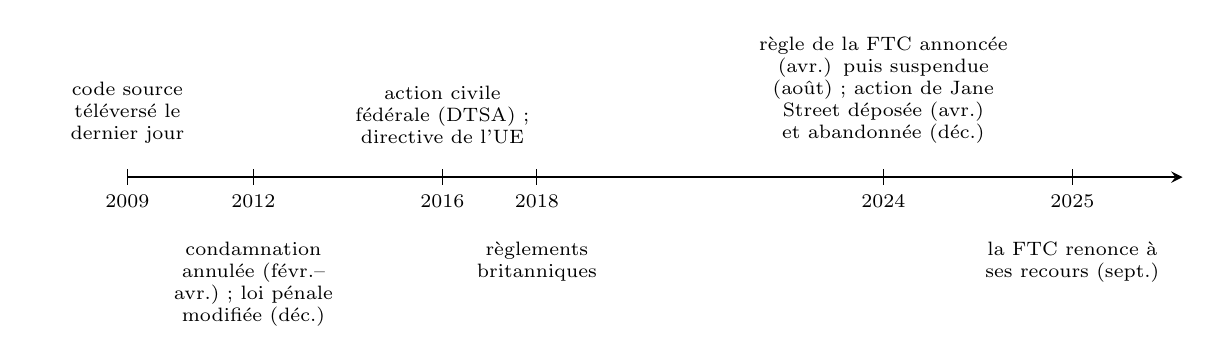
\begin{tikzpicture}[font=\scriptsize,>=stealth]
\draw[->,thick] (0,0) -- (13.4,0);
\foreach \x/\y in {0/2009,1.6/2012,4.0/2016,5.2/2018,9.6/2024,12.0/2025} {\draw (\x,0.1) -- (\x,-0.1) node[below] {\y};}
\node[align=center,anchor=south,text width=2.3cm] at (0,0.3) {code source téléversé le dernier jour};
\node[align=center,anchor=north,text width=2.6cm] at (1.6,-0.7) {condamnation annulée (févr.--avr.)~; loi pénale modifiée (déc.)};
\node[align=center,anchor=south,text width=2.3cm] at (4.0,0.3) {action civile fédérale (DTSA)~; directive de l'UE};
\node[align=center,anchor=north,text width=2.0cm] at (5.2,-0.7) {règlements britanniques};
\node[align=center,anchor=south,text width=3.6cm] at (9.6,0.3) {règle de la FTC annoncée (avr.) puis suspendue (août)~; action de Jane Street déposée (avr.) et abandonnée (déc.)};
\node[align=center,anchor=north,text width=2.4cm] at (12.0,-0.7) {la FTC renonce à ses recours (sept.)};
\end{tikzpicture}

\omcaption{Le dossier public du chapitre~: l'affaire pénale du hook et la modification qui a suivi, les textes civils, l'essor puis le recul de
la règle fédérale sur les \omterm{def:fm:intellectual-property-and-non-competes:restrict}{clauses de non-concurrence}, et un litige civil qui s'est achevé sans jugement au fond. Sources~: le registre du chapitre.}\label{fig:fm:intellectual-property-and-non-competes:record}
\end{omfigure}

\begin{method}[Protéger ce qui part avec les personnes]\label{met:fm:intellectual-property-and-non-competes:protect}
\begin{enumerate}
\item Inventorier ce que la société possède dans les trois catégories (structure, paramètres, données) et estimer la vitesse à laquelle chacune perd de sa valeur une fois sorties.
\item Prendre les mesures raisonnables~: accès limité au besoin d'en connaître, copies et envois journalisés, séparation des tâches, \omterm{def:fm:intellectual-property-and-non-competes:nda}{accord de confidentialité} et \omterm{def:fm:intellectual-property-and-non-competes:nda}{clause de cession des
inventions} dans chaque contrat.
\item Fixer la durée du préavis et des restrictions selon le type de connaissance (\cref{prop:fm:intellectual-property-and-non-competes:six}), dans la limite de ce que
le droit local permet, et les rémunérer.
\item Au moment de chaque départ~: couper l'accès dès la démission, examiner les journaux et rappeler par écrit au salarié ses obligations.
\item Demander un avis juridique avant de s'appuyer sur une restriction ou d'engager une action en justice.
\end{enumerate}
\end{method}

\section{Construction~: le calculateur de garden leave}\label{bld:fm:intellectual-property-and-non-competes:gardenleave}

\begin{build}
\bfield{Rôle} Aucune construction honnête~: le sujet du chapitre est juridique. L'outil d'analyse évalue une restriction comme un actif qui se déprécie face à son
coût salarial.
\bfield{Interface} \texttt{firm.gardenleave}~: \texttt{loss\_if\_start}, \texttt{protected}, \texttt{leave\_cost}, \texttt{net}, \texttt{best\_length},
\texttt{half\_life\_from\_series} (enveloppe de \texttt{firm.decay.half\_life\_fit}).
\bfield{Règles} La valeur protégée plus la perte restante égale la perte sans restriction~; la meilleure durée maximise la valeur nette et ne dépend
pas du taux d'actualisation~; aucune restriction ne vaut la peine lorsque $LP\le S$.
\bfield{Tests d'acceptation} \texttt{code/firm/gardenleave/tests/}~: l'identité, la meilleure durée comparée à une recherche sur grille, et la demi-vie d'une
décroissance propre.
\bfield{Pour aller plus loin} Un concurrent qui a besoin de temps pour se reconstituer~; une probabilité que la restriction ne soit pas appliquée~; le coût espéré d'une fuite comparé au
coût de la mise en œuvre d'une action en justice.
\end{build}

\begin{omsources}
\item United States v. Aleynikov, 676 F.3d 71 (2d Cir. 2012)~; Theft of Trade Secrets Clarification Act of 2012, Pub.~L.~112-236.
\item 18 U.S.C. 1836 et 1839~; Directive (UE) 2016/943~; The Trade Secrets (Enforcement, etc.) Regulations 2018 (SI 2018/597).
\item Federal Trade Commission, Noncompete Rule page et communiqué de presse de septembre 2025.
\item Jane Street Group, LLC v. Millennium Management LLC et al., n°~1:24-cv-02783 (S.D.N.Y.), plainte et stipulation de désistement.
\end{omsources}

\section{Exercices}

\begin{exercise}[$\star$]\label{exo:fm:intellectual-property-and-non-competes:1}
Dans l'\cref{ex:fm:intellectual-property-and-non-competes:hand}, calculer la valeur protégée par six et douze mois de congé et la perte sans
congé.
\end{exercise}

\begin{exercise}[$\star$]\label{exo:fm:intellectual-property-and-non-competes:2}
Énumérer les trois conditions pour qu'une information soit un \omterm{def:fm:intellectual-property-and-non-competes:secret}{secret des affaires}. Un signal décrit dans un article publié est-il un \omterm{def:fm:intellectual-property-and-non-competes:secret}{secret des affaires}~? La version ajustée par la société
de ce signal l'est-elle~?
\end{exercise}

\begin{exercise}[$\star$]\label{exo:fm:intellectual-property-and-non-competes:3}
Combien coûte un \omterm{def:fm:intellectual-property-and-non-competes:restrict}{garden leave} de trois, six et douze mois à 1.5~million de dollars par an, actualisé à 8~\%~?
\end{exercise}

\begin{exercise}[$\star\star$]\label{exo:fm:intellectual-property-and-non-competes:4}
Pour quelle demi-vie six mois est-il la meilleure durée lorsque $LP/S=8$~? Lorsque $LP/S=4$~?
\end{exercise}

\begin{exercise}[$\star\star$]\label{exo:fm:intellectual-property-and-non-competes:5}
Pourquoi la condamnation du hook a-t-elle été annulée, et qu'a modifié le Congrès en 2012~?
\end{exercise}

\begin{exercise}[$\star\star$]\label{exo:fm:intellectual-property-and-non-competes:6}
Établir la valeur nette à la meilleure durée avec $r=0$ et la vérifier sur l'\cref{ex:fm:intellectual-property-and-non-competes:hand}.
\end{exercise}

\begin{exercise}[$\star\star\star$]\label{exo:fm:intellectual-property-and-non-competes:7}
\emph{Programmation.} Relancer \texttt{fm\_ip.table(seed=12)}. Que deviennent les demi-vies et les meilleures durées~?
\end{exercise}

\begin{exercise}[$\star\star\star$]\label{exo:fm:intellectual-property-and-non-competes:8}
\emph{Trouver la faille.} «~La structure de notre modèle est la partie qui a de la valeur. Une \omterm{def:fm:intellectual-property-and-non-competes:restrict}{clause de non-concurrence} de deux ans la protège entièrement.~»
\end{exercise}

\section{Problème~: La question des six mois}

\begin{problem}[{Problème du week-end --- la question des six mois}]\label{pb:fm:intellectual-property-and-non-competes:1}
Un chercheur senior d'une stratégie qui rapporte 20~millions de dollars par an démissionne pour rejoindre un concurrent. Le responsable du desk doit décider de ce qu'il protège et
pendant combien de temps il tient le chercheur à l'écart du marché.

\medskip\noindent\textbf{Partie I --- Ce que la société possède.}
\begin{enumerate}
\item Lister ce qu'une société de trading possède et qu'un concurrent ne peut pas acheter.
\item Pourquoi les brevets et le droit d'auteur protègent-ils si peu de chose~?
\item Définir un \omterm{def:fm:intellectual-property-and-non-competes:secret}{secret des affaires} et nommer la condition que la société contrôle.
\item Définir un \omterm{def:fm:intellectual-property-and-non-competes:nda}{accord de confidentialité} et une \omterm{def:fm:intellectual-property-and-non-competes:nda}{clause de cession des inventions}.
\end{enumerate}

\medskip\noindent\textbf{Partie II --- Le droit.}
\begin{enumerate}[resume]
\item Résumer les faits et l'issue de l'affaire United States v. Aleynikov.
\item Qu'a modifié l'amendement de 2012, et qu'a ajouté la loi de 2016~?
\item Où en est la règle de la FTC sur les \omterm{def:fm:intellectual-property-and-non-competes:restrict}{clauses de non-concurrence}~?
\item Que reprochait la plainte contre Jane Street, et comment l'affaire s'est-elle terminée~?
\end{enumerate}

\medskip\noindent\textbf{Partie III --- Le modèle.}
\begin{enumerate}[resume]
\item Définir une \omterm{def:fm:intellectual-property-and-non-competes:restrict}{clause de non-concurrence}, le \omterm{def:fm:intellectual-property-and-non-competes:restrict}{garden leave} et une \omterm{def:fm:intellectual-property-and-non-competes:restrict}{clause de non-sollicitation}.
\item Écrire la valeur protégée et le coût d'une restriction de durée $T$.
\item Énoncer et démontrer la \cref{prop:fm:intellectual-property-and-non-competes:six}.
\item Donner les demi-vies ajustées des trois types de connaissance.
\item Donner la valeur protégée par six mois pour chacune, et sa part de la perte sans \omterm{def:fm:intellectual-property-and-non-competes:restrict}{garden leave}.
\item Donner les meilleures durées, et expliquer pourquoi chacune correspond à autant de demi-vies.
\end{enumerate}

\medskip\noindent\textbf{Partie IV --- La décision.}
\begin{enumerate}[resume]
\item Le chercheur connaît la structure et les paramètres. Quelle restriction faudrait-il imposer, et qu'apportent six mois~?
\item Qu'est-ce qui protège la structure au-delà de toute restriction~?
\item Lister les étapes à suivre le jour de la démission.
\item Dans quelle mesure les meilleures durées sont-elles robustes au bruit dans les estimations de demi-vie~?
\item Énoncer le \emph{résultat nommé}~: la durée de \omterm{def:fm:intellectual-property-and-non-competes:restrict}{garden leave} pour laquelle l'avantage marginal protégé égale le coût salarial marginal.
\item En deux phrases, rédiger la politique de la société en matière de restrictions.
\end{enumerate}
\end{problem}

\section{Questions d'entretien}

\begin{interviewq}[$\star$ \iqroles{chercheur, trader}]\label{iq:fm:intellectual-property-and-non-competes:1}
Qu'est-ce que le \omterm{def:fm:intellectual-property-and-non-competes:restrict}{garden leave}, et pourquoi une société vous paierait-elle pour ne pas travailler~?
\end{interviewq}

\begin{interviewq}[$\star$ \iqroles{développeur}]\label{iq:fm:intellectual-property-and-non-competes:2}
Vous avez écrit une bibliothèque de backtesting dans votre dernier poste. Pouvez-vous l'emporter avec vous~?
\end{interviewq}

\begin{interviewq}[$\star\star$ \iqroles{chercheur}]\label{iq:fm:intellectual-property-and-non-competes:3}
La valeur d'un signal est divisée par deux tous les six mois. Quelle part de celle-ci une \omterm{def:fm:intellectual-property-and-non-competes:restrict}{clause de non-concurrence} de six mois protège-t-elle~?
\end{interviewq}

\begin{interviewq}[$\star\star$ \iqroles{risque}]\label{iq:fm:intellectual-property-and-non-competes:4}
Que journaliseriez-vous pour montrer que la société prend des mesures raisonnables pour garder son code secret~?
\end{interviewq}

\begin{interviewq}[$\star\star$ \iqroles{chercheur}]\label{iq:fm:intellectual-property-and-non-competes:5}
Lequel se dévalue-t-il le plus vite~: les paramètres d'un modèle ou sa structure~? Quelles conséquences pour les contrats d'une société~?
\end{interviewq}

\begin{interviewq}[$\star\star\star$ \iqroles{chercheur, trader}]\label{iq:fm:intellectual-property-and-non-competes:6}
Dérivez la durée de \omterm{def:fm:intellectual-property-and-non-competes:restrict}{garden leave} qui maximise sa valeur nette pour la société.
\end{interviewq}
